%%%% fs-run-mapreduce Optimistic collision management
\label {fs-collision}

As it was defined previously, only grouping depends on the input order, because it maintains state. Therefore, we assumed, that data items flow through the operations in the right order. However, this restriction is hard to satisfy, because of asynchrony and possible existence of multiple paths between two nodes.

In order to figure out this issue, we accept the fact that grouping can produce incorrect tuples. However, we require that {\it all correct tuples are eventually produced}. The correctness of tuple means that this tuple would be generated if the order assumption was satisfied. 

To eventually produce all correct tuples, we use approach called {\it replay}. If the item gets in grouping, according to the meta-information order, nothing is replayed and only the most recent window is produced. If the item is out-of-order, it is inserted in the bucket at the correct location, and all tuples, which contain this element, are reproduced. Thereby, replay guarantees that eventually all correct tuples are generated.

The example of replay is shown on the figure~\ref{grouping-replaying-figure}. In this example the green item is out-of-order and the window of grouping is 2.

\begin{figure}[htbp]
  \centering
  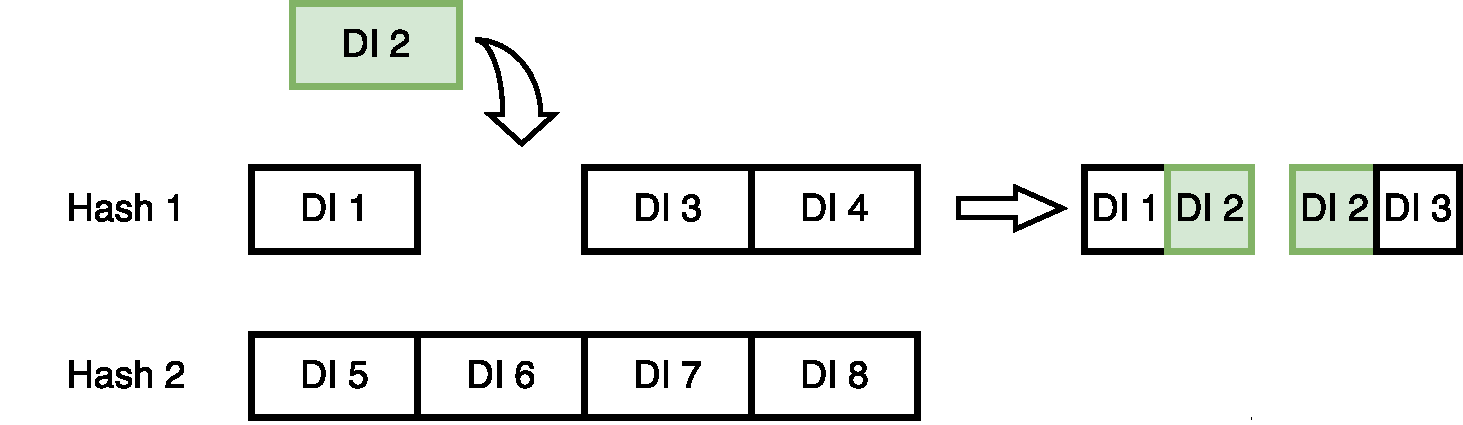
\includegraphics[width=0.48\textwidth]{pics/grouping-replaying}
  \caption{Replay in grouping}
  \label {grouping-replaying-figure}
\end{figure}

In the case of the right order of the input items, there is no redundant items produced. Nevertheless, our optimistic approach can lead to the generation of invalid elements in the stream that should not be send to the outer world. The next section details the solution of this issue.
